\begin{frame}
\centering
\Large
Requirements
\end{frame}

\begin{frame}{Requirements}
    \begin{itemize}
        \item Get model information from user
        \item Convert user input to usable data
        \item Create \emph{dynamic} LCI model
        \item Calculate resulting impact
        \item Provide feedback of results
    \end{itemize}
\end{frame}







\begin{frame}{Traditional Aggregation}

\vfill
\begin{figure}
    \centering
    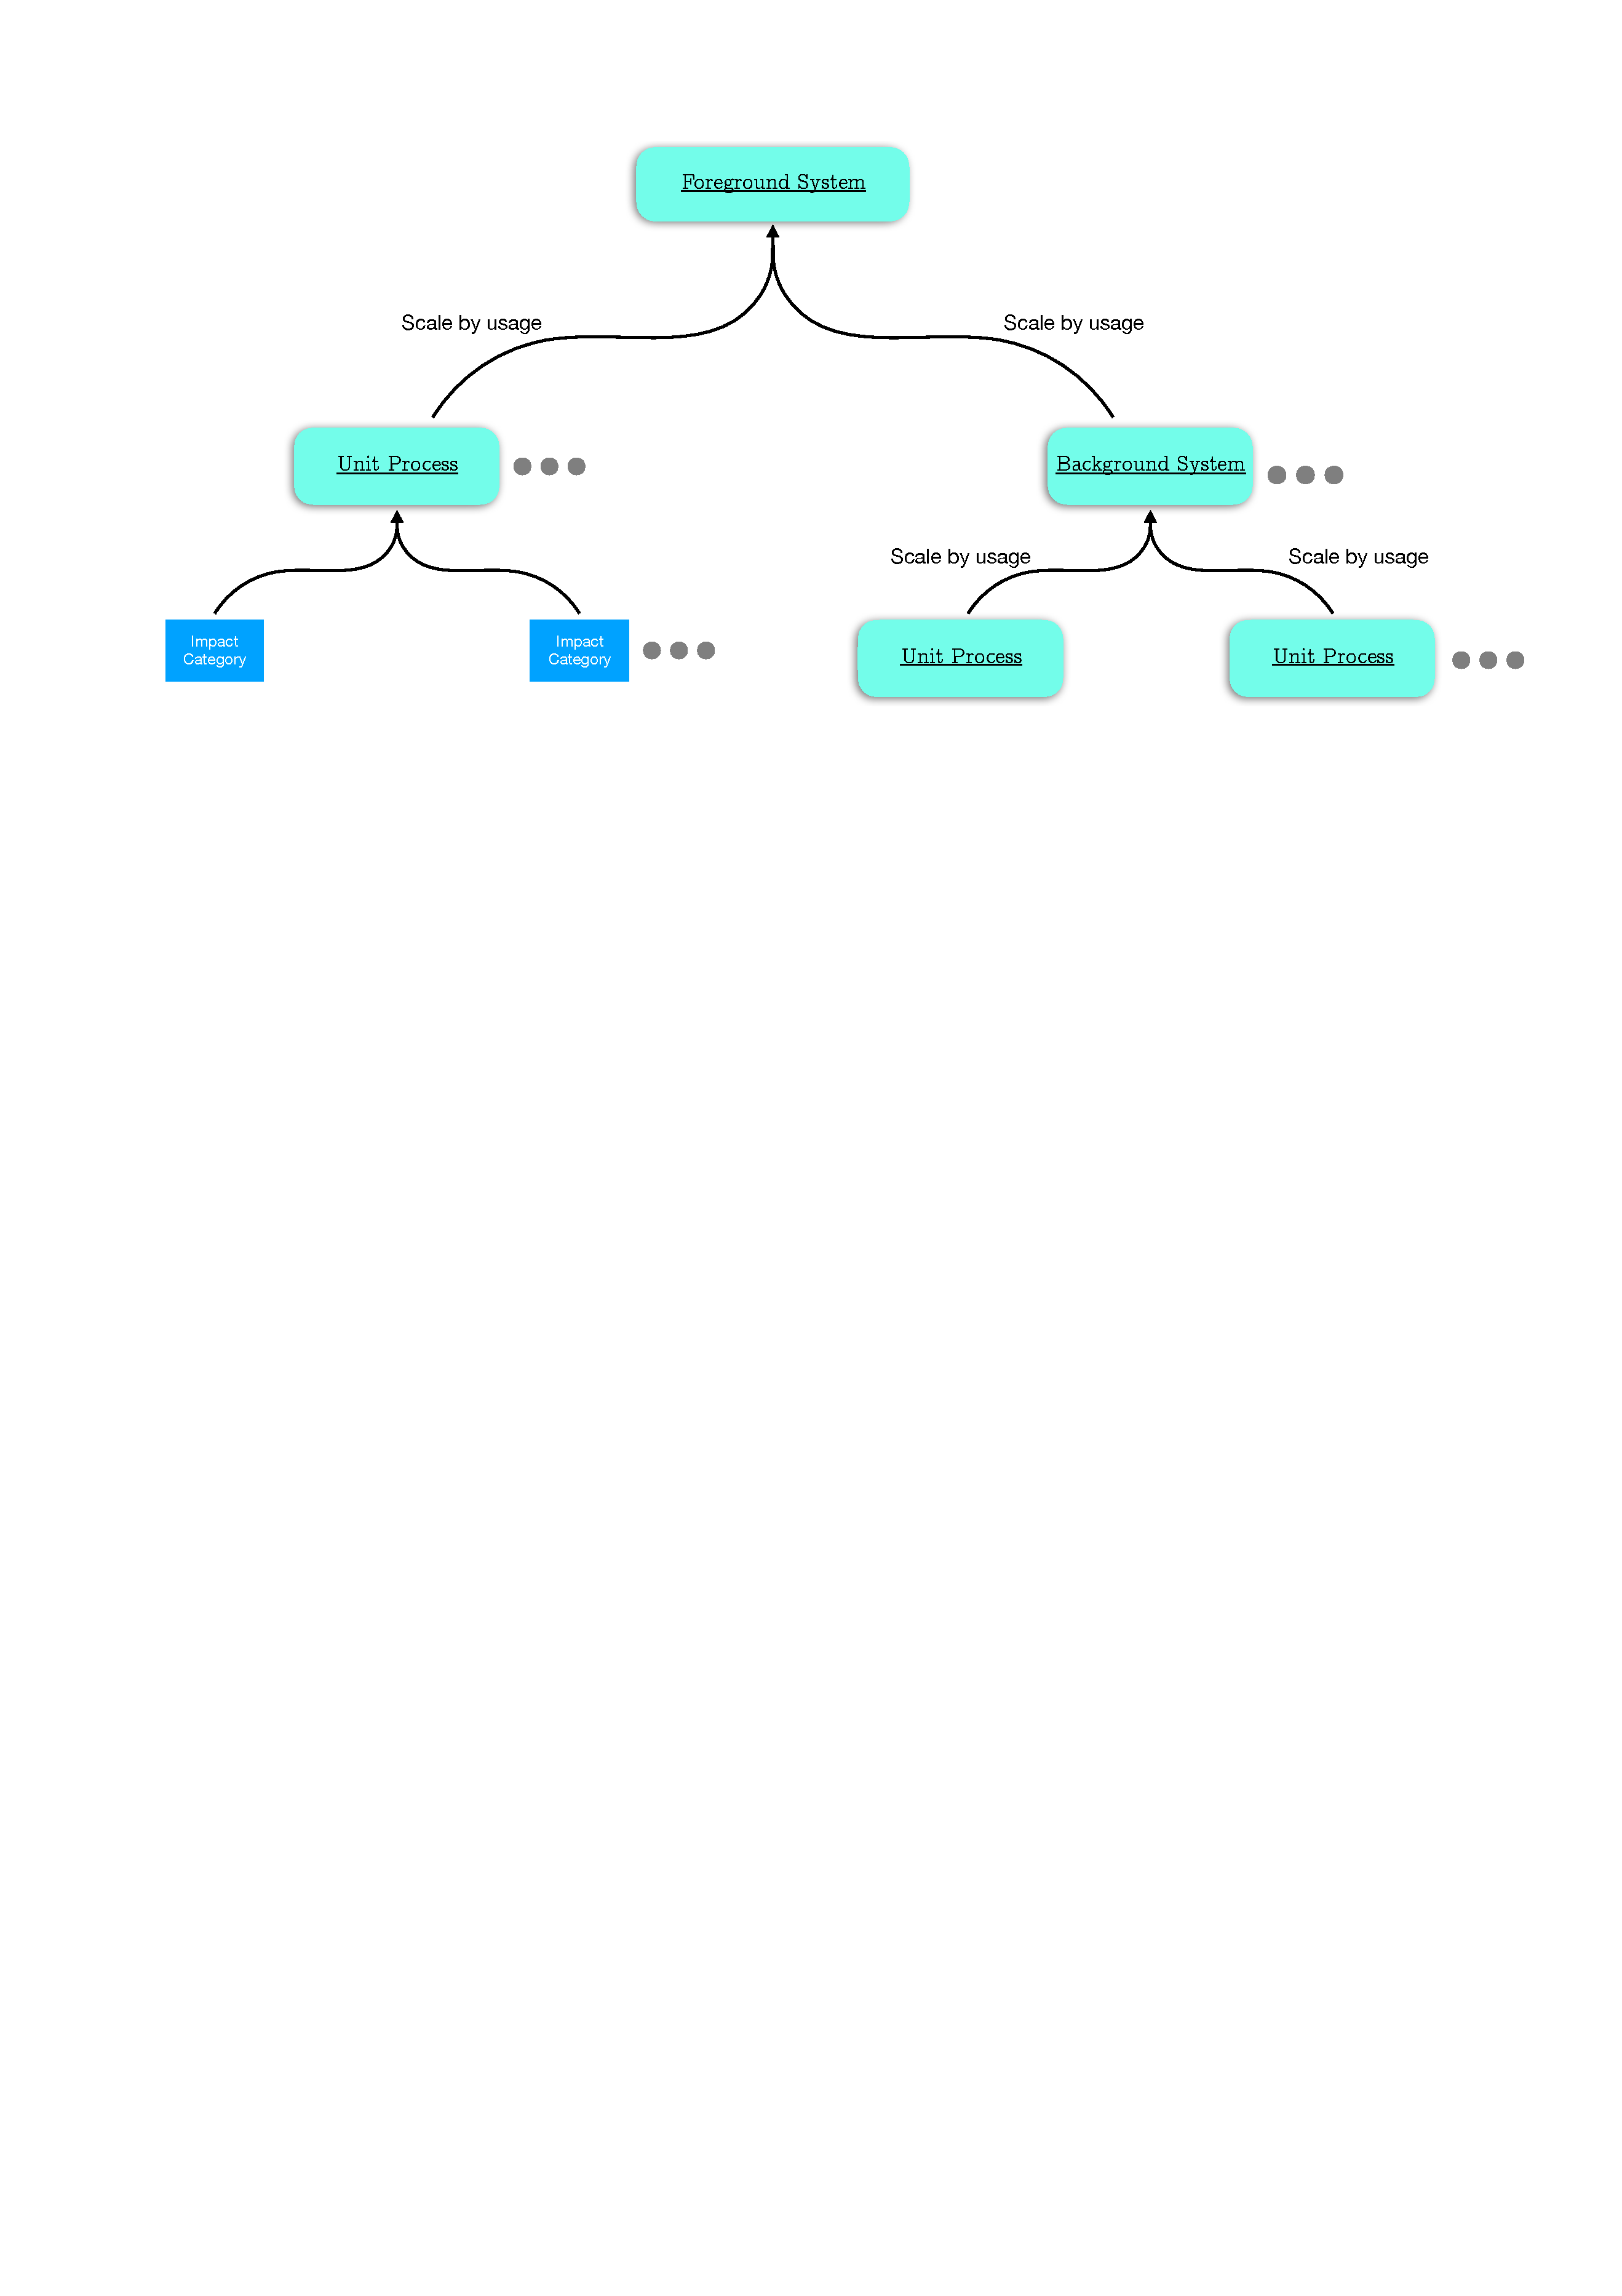
\includegraphics[page=1, width = \linewidth]{.figures/ImpactAggregationExtension.pdf}
\end{figure}

\end{frame}

\begin{frame}{Extended Aggregation}
\vfill
Extensions: Timestamped data values and dynamic properties.
\vfill
\begin{figure}
    \centering
    \includegraphics[page=2, width = \linewidth]{.figures/ImpactAggregationExtension.pdf}
\end{figure}

\end{frame}